% Created 2024-07-08 Mon 22:16
% Intended LaTeX compiler: pdflatex
\documentclass[11pt]{article}
\usepackage[utf8]{inputenc}
\usepackage[T1]{fontenc}
\usepackage{ragged2e}
\usepackage{caladea}
\usepackage{graphicx}
\usepackage{longtable}
\usepackage{wrapfig}
\usepackage{rotating}
\usepackage{epigraph}
\usepackage[normalem]{ulem}
\usepackage{hyperref}
\usepackage{amsmath}
\usepackage{amssymb}
\usepackage{capt-of}
\usepackage{hyperref}
\usepackage{fancyhdr}
\title{Novena à Santa Bibiana}
 % \hypersetup{
 %  pdfauthor={},
 %  pdftitle={Novena a/à SANTO_NOME},
 %  pdfkeywords={},
 %  pdfsubject={},
 %  pdfcreator={Emacs 29.4 (Org mode 9.6.15)}, 
 %  pdflang={English}
 % }

\title{
  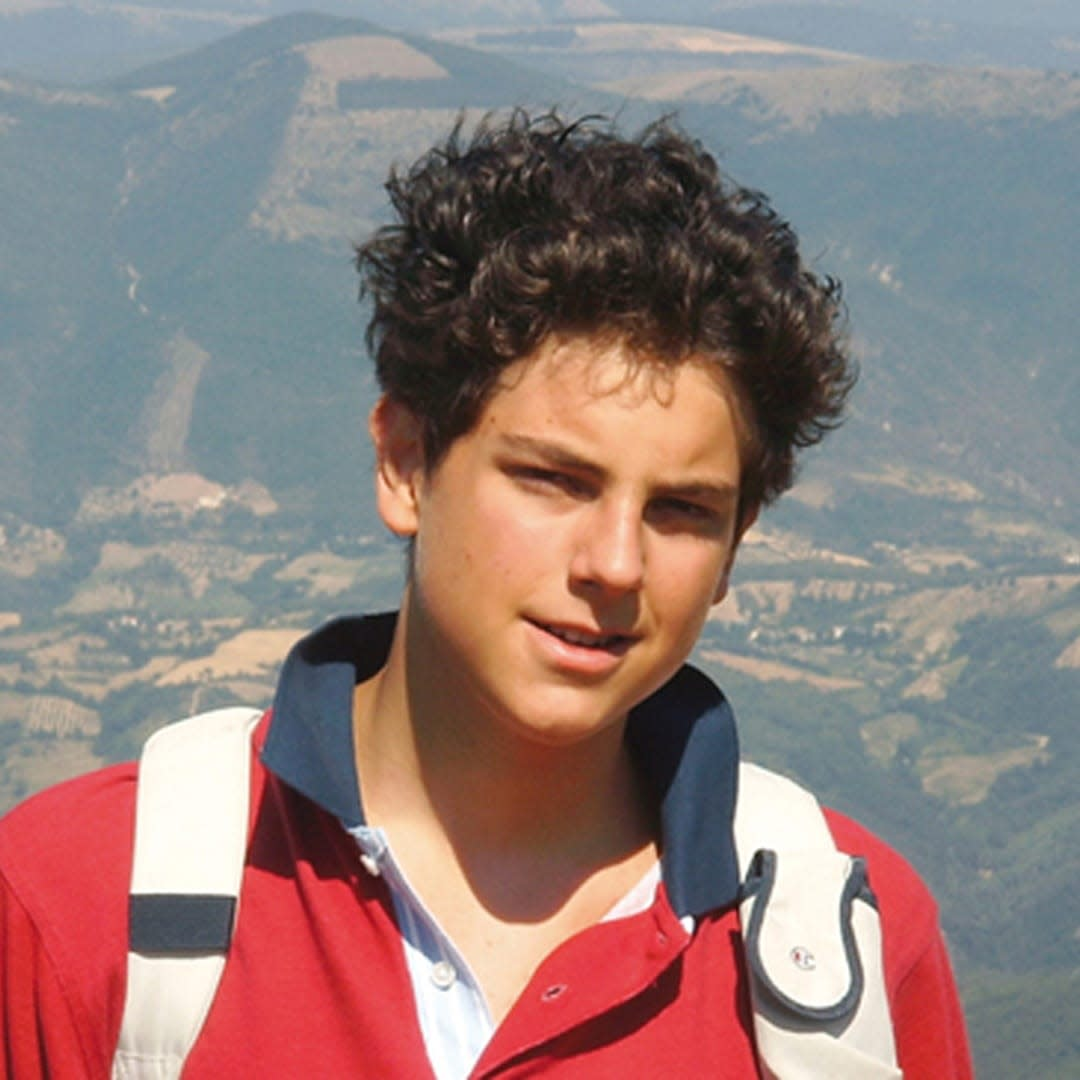
\includegraphics[scale=0.23]{./assets/imagem.jpg}
  \par
   NOVENA A SANTA FRANCISCA XAVIER CABRINI }
\author{Garamog, Nina Freitas}
\date{13/12 - 22/12}
\renewcommand{\contentsname}{Sumário}

\begin{document}


\thispagestyle{empty}

\pagestyle{fancy}
\fancyhf{} % clear existing header/footer entries
\fancyfoot[LO, CE]{
  
\includegraphics[scale=0.2]{./assets/cross.png}}
% Place Page X of Y on the right-hand
% side of the footer
\fancyfoot[R]{\thepage}
  
\newpage

\tableofcontents

\centering
\vfill
Visite-nos no Telegram: \url{https://t.me/CotidieNovena}
\newpage


%%%%%%%%%%%%%%%%%%%%%%%%%%%%%%%%%%%%% Orações  %%%%%%%%%%%%%%%%%%%%%%%%%%%%%%%%%%%%%%%%%%%

\section{Primeiro Dia}
\subsection{Reflexão}
Prepararei um confortável berço ao Deus Menino, com atos de profunda humildade: nunca uma palavra em meu louvor, nunca um pensamento favorecido pela soberba satisfação, não desculparei a mim mesmo, não teimarei em defender a minha opinião, não inventarei pretextos para salvar o meu amor próprio. Repetirei o tempo todo aquela frase que formou muitos santos: "Do zero para cima, tudo é de Deus - do zero para baixo, sou exatamente eu". O meu coração se tornará, assim, um berço macio, no qual o Santo Menino se deitará feliz.

\subsection{Jaculatória}
Como és belo, doce Menininho,
Mesmo deitado entre o boi e o burrinho!
Mas vou fazer-te mais belo e mais elegante,
Se em mim vier descansar-te.
\textbf{Pai-Nosso, Avé-Maria, Glória ao Pai... }

\section{Segundo Dia}
\subsection{Reflexão}
A candura da mente, a pureza do coração, a modéstia dos atos exteriores representarão para o Menino Jesus uma macia e cândida camisa. Por isso, evitarei hoje todo pecado venial percebido.
\subsection{Jaculatória}
Pecado feio, mais não te quero,
Porque ao meu Jesus faz cair no choro!
\textbf{Pai-Nosso, Avé-Maria, Glória ao Pai... }

\section{Terceiro Dia}
\subsection{Reflexão}
A amabilidade no rosto, na palavra, no olhar e no sorriso, a serena calma nos encontros e desencontros da vida, o cuidado de ver em tudo o lado belo e bom, e de infundir em cada coração alegria e paz, formarão para o Petiz de Belém um sedoso colchãozinho de celeste macieza. Hoje, suportarei em paz cada áspero e duro acontecimento.
\subsection{Jaculatória}
Hoje, quero mesmo atento estar,
Para Tua Mãe, de mim, contente ficar.
E, então, estarei certo que Tu também,
ó meu pequeno Jesus, me quererás bem!
\textbf{Pai-Nosso, Avé-Maria, Glória ao Pai... }

\section{Quarto Dia}
\subsection{Reflexão}
Para cobrir a cabecinha adorada de Jesus Menino, terei em minha mente apenas pensamentos celestes, afastarei prontamente todo inútil fantasma e vigiarei a pureza de cada intenção, esforçando-me de dar a cada ato, mesmo o mais ínfimo, um fim sobrenatural e santo. Ao cobrir a cabeça de Jesus, pedir-lhe-ei um olhar de misericórdia para os pobres pecadores e lhe consagrarei todo o meu coração.
\subsection{Jaculatória}
Dai-me, ó Maria, na Hóstia do amor
O Divino Petiz do meu coração.
\textbf{Pai-Nosso, Avé-Maria, Glória ao Pai... }

\section{Quinto Dia}
\subsection{Reflexão}
Hoje, voarei leve como pluma ao primeiro aceno da obediência e cumprirei com cuidadosa precisão os meus deveres, mesmo que sejam repugnantes para as minhas tendências e os meus desejos. Não terei, hoje, nenhuma hesitação nem discutirei as ordens que eu receber: sorrirei generosamente ao sacrifício, a fim de que o Santo Menino durma sonhos imperturbados e serenos sobre a suave pluma de meu dom de amor.
\subsection{Jaculatória}
Hoje, voarei leve como pluma ao primeiro aceno da obediência e cumprirei com cuidadosa precisão os meus deveres, mesmo que sejam repugnantes para as minhas tendências e os meus desejos. Não terei, hoje, nenhuma hesitação nem discutirei as ordens que eu receber: sorrirei generosamente ao sacrifício, a fim de que o Santo Menino durma sonhos imperturbados e serenos sobre a suave pluma de meu dom de amor.
\textbf{Pai-Nosso, Avé-Maria, Glória ao Pai... }

\section{Sexto Dia}
\subsection{Reflexão}
Para preparar belas fraldas ao infante Divino, farei um esforço para vigiar a minha língua, evitando palavras ociosas, conversas amargas e profanas, e aquela frívola loquacidade que é o túmulo da vida interior. Hoje, calar-me-ei, sobretudo, nos momentos mais difíceis, nas reprimendas não merecidas, imolando as minhas razões no meu amável Jesus, que se fez silêncio por amor.

\subsection{Jaculatória}
O caro, santo silêncio de ouro
quero guardar como um tesouro.
\textbf{Pai-Nosso, Avé-Maria, Glória ao Pai... }

\section{Sétimo Dia}
\subsection{Reflexão}
Cobrirei afetusoamente o Santo Menino com os lençóis macios da devoção; olharei sempre para Ele, estudarei, trabalharei, me divertirei sob o olhar de Jesus, me mortificarei por Jesus, a Ele elevarei perenemente o cântico da piedade, com frequentes jaculatórias e comunhões espirituais. A cada hora, o meu pensamento irá a Jesus e Maria e vice-versa, para que toda a minha vida se conforme às Suas virtudes.

\subsection{Jaculatória}
Com minhas florzinhas e minhas ervinhas
Vou perfurmar-Te os frios lençoizinhos,
Ó caro Menininho da alma minha,
Suprema doçura e poesia minha!
\textbf{Pai-Nosso, Avé-Maria, Glória ao Pai... }

\section{Oitavo Dia}
\subsection{Reflexão}
Generosa mortificação da mente, do coração e do corpo bordará o cobertorzinho do Infante Jesus: a lembrança dEle inocente e imolado à Justiça Divina por causa dos meus pecados, me deixará atento e livre de sacrificar a natureza às exigências da reparação. Direi sempre 'sim' a Jesus e 'não' a mim mesmo, e transformarei cada espinho da vida em uma rosa de amor, que despetalarei aos pés da santa colina para fazer Jesus sorrir.

\subsection{Jaculatória}
Aqui são espinhos todas as coisas,
Somente com Deus desabrocham as rosas!
\textbf{Pai-Nosso, Avé-Maria, Glória ao Pai... }

\section{Nono Dia}
\subsection{Reflexão}
Completarei o enxoval de Jesus com um lencinho cuidadosamente bordado, que servirá para enxugar as Suas primeiras lágrimas. Jesus chora porque não é amado. Portanto, hoje, terei o cuidado de fazer cada ação por puro amor, não por cálculos humanos ou vantagem pessoal, mas apenas para consolá-Lo e dar alegrias a Seu Coração. Aprenderei a sofrer interiormente em silêncio sem cessar de sorrir.

\subsection{Jaculatória}
O mundo todo conduzir a Ti eu gostaria,
Ó sol esplendido dos olhos meus,
Gostaria que todos no Paraíso
Provassem um belo dia de Teu sorriso.


\section{Oferecimento do Enxovalzinho a Jesus pelas mãos de Maria}
Santíssima Virgem, o pequeno pacote que desejo apresentar ao Menino Jesus está pronto na pobre cela de meu coração, mas é tão imperfeito que não tenho a coragem de lho oferecer. Tu, que com tuas delicadíssimas mãos maternas preparaste para Jesus um cândido enxovalzinho perfumado de Paraíso, debruça-te sobre meu pobre trabalho, purifica-o com teu olhar, inflamá-o com as batidas de Teu Coração Imaculado, para que possa ser aceito pelo pequeno Jesus, e Ele venha a nascer no meu coração, onde proponho guardá-Lo e amá-Lo como único tesouro. 


Pelas Tuas mãos, dulcíssima Maria,
Terei a Jesus, delícia e vida minha!

\textbf{Pai-Nosso, Avé-Maria, Glória ao Pai... }

\subsection*{Créditos:}
\href{https://precantur.blogspot.com/2011/12/novena-do-enxovalzinho-do-menino-jesus.html}{Thesaurus Precum}


\end{document}
